\documentclass{article}
\usepackage{amsmath}
\usepackage{tikz}
\usetikzlibrary{positioning}
\usetikzlibrary{calc}

\usepackage{circuitikz}
\usetikzlibrary{circuits.logic.IEC,calc}

\begin{document}


\begin{tikzpicture}[
    fulladder/.style={draw, minimum size=3cm,
    label={[xshift=8mm]left:$c_\text{out}$},
    label={[yshift=5mm]below:$s$},
    label={[xshift=-6mm]right:$c_\text{in}$},
    label={[yshift=-3mm, anchor=center]65:$b$},
    label={[yshift=-3mm, anchor=center]115:$a$},
    }]

    \node[fulladder] (a) {F.A};
    \node[fulladder, right=1cm of a] (b) {F.A};

    \draw[<-] (a.115) --++(90:0.5cm) node [above] {$a_1$};
    \draw[<-] (a.65) --++(90:0.5cm) node [above] {$b_1$};
    \draw[<-] (b.115) --++(90:0.5cm) node [above] {$a_0$};
    \draw[<-] (b.65) --++(90:0.5cm) node [above] {$b_0$};
    \draw[<-] (b.east) --++(0:0.5cm) node [right] {$0$};
    \draw[<-] (a.east) -- (b.west);
    \draw[->] (a.west) --++(180:0.5cm) node [left] {$c$};
    \draw[->] (a.south) --++(-90:0.5cm) node [below] {$s_1$};
    \draw[->] (b.south) --++(-90:0.5cm) node [below] {$s_0$};
\end{tikzpicture}





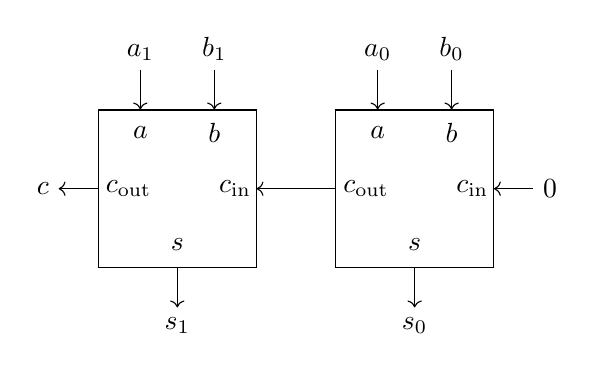
\begin{tikzpicture}[
    fulladder/.style={draw, minimum size=2cm,
    label={[xshift=8mm]left:$c_\text{out}$},
    label={[yshift=5mm]below:$s$},
    label={[xshift=-6mm]right:$c_\text{in}$},
    label={[yshift=-3mm, anchor=center]65:$b$},
    label={[yshift=-3mm, anchor=center]115:$a$},
    }]

    \node[fulladder] (a) {};
    \node[fulladder, right=1cm of a] (b) {};

    \draw[<-] (a.115) --++(90:0.5cm) node [above] {$a_1$};
    \draw[<-] (a.65) --++(90:0.5cm) node [above] {$b_1$};
    \draw[<-] (b.115) --++(90:0.5cm) node [above] {$a_0$};
    \draw[<-] (b.65) --++(90:0.5cm) node [above] {$b_0$};
    \draw[<-] (b.east) --++(0:0.5cm) node [right] {$0$};
    \draw[<-] (a.east) -- (b.west);
    \draw[->] (a.west) --++(180:0.5cm) node [left] {$c$};
    \draw[->] (a.south) --++(-90:0.5cm) node [below] {$s_1$};
    \draw[->] (b.south) --++(-90:0.5cm) node [below] {$s_0$};
\end{tikzpicture}






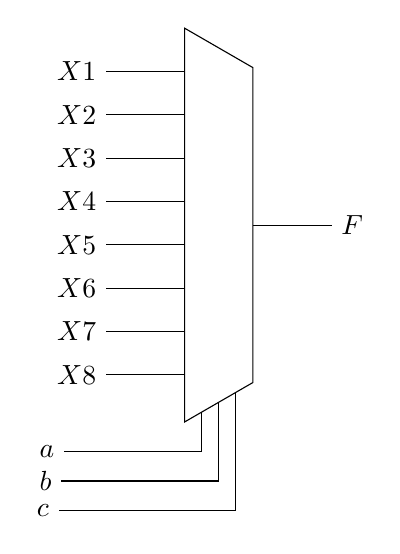
\begin{tikzpicture}
\draw (0,0)coordinate (O)--++(30:1)coordinate (A)--++(90:4)coordinate (B)--++(150:1)coordinate (C)--cycle;
\draw ($(A)!0.5!(B)$)--++(0:1)node[right]{$F$};
\draw ($(O)!0.5!(A)$)--++(-90:1)--++(180:2)node[left]{$b$};
\draw ($(O)!0.25!(A)$)--++(-90:0.5)--++(180:1.75)node[left]{$a$};
\draw ($(O)!0.75!(A)$)--++(-90:1.5)--++(180:2.25)node[left]{$c$};
\foreach \y/\t in {0.1/1,0.2/2,0.3/3,0.4/4,0.5/5,0.6/6,0.7/7,0.8/8} {
\draw ($(C)! \y*1.1 !(O)$)--++(180:1) node[left] {$X \t$};}
\end{tikzpicture}












\begin{circuitikz}[circuit logic IEC] 
\node[and gate,inputs={nnnnnnnn},and gate IEC symbol={},text height=3cm,
] (A) {};
\foreach \Valor in {1,...,8}
{
  \draw  ([xshift=-10pt]A.input \Valor) node[left] {$I_{\Valor}$} -- (A.input \Valor);
}
\draw (A.output) -- ++(10pt,0) node[right] {$F$};
\draw ( $ (A.south west)!0.25!(A.south east) $ ) -- ++(-90:0.25) |- ++(-10pt,0) node[left] {$a$};
\draw (A.south) -- ++(-90:0.5) |- ++(-15pt,0) node[left] {$b$};
\draw ( $ (A.south west)!0.75!(A.south east) $ ) -- ++(-90:0.75) |- ++(-20pt,0) node[left] {$c$};
\end{circuitikz}





\begin{circuitikz}
 \ctikzset{tripoles/en amp/input height=0.45}
 \draw (0,0)node[en amp](E){}
 (E.out) node[right] {$v_{\mathrm{out}}$}
 (E.-) node[left] {$v_{\mathrm{in}-}$}
 (E.+) node[left] {$v_{\mathrm{in}+}$};
 \end{circuitikz}





\begin{circuitikz} \draw
 (0,2) node[and port] (myand1) {}
 (0,0) node[and port] (myand2) {}
 (2,1) node[xnor port] (myxnor) {}
 (myand1.out) -| (myxnor.in 1)
 (myand2.out) -| (myxnor.in 2)
 ;\end{circuitikz}






\begin{circuitikz}
 \ctikzset{multipoles/thickness=4}
 \ctikzset{multipoles/external pins thickness=2}
 \draw (0,0) node[dipchip,
 num pins=12,
 hide numbers,
 external pins width=0.3,
 external pad fraction=4 ](C){IC1};
 \draw (C.pin 1) -- ++(-0.5,0) to[R]
 ++(0,-3) node[ground]{};
 \node [right, font=\tiny]
 at (C.bpin 1) {RST};
 \end{circuitikz}







\begin{circuitikz}
 \ctikzset{multipoles/thickness=3}
 \ctikzset{multipoles/dipchip/width=2}
 \draw (0,0) node[dipchip,
 num pins=10, hide numbers, no topmark,
 external pins width=0](C){Block};
 \node [right, font=\tiny] at (C.bpin 1) {RST};
 \node [right, font=\tiny] at (C.bpin 2) {IN1};
 \node [right, font=\tiny] at (C.bpin 4) {/IN2};
 \node [left, font=\tiny] at (C.bpin 8) {OUT};
 \draw (C.bpin 2) -- ++(-0.5,0) coordinate(extpin);
 \node [ocirc, anchor=0](notin2) at (C.bpin 4) {};
 \draw (notin2.180) -- (C.bpin 4 -| extpin);
 \draw (C.bpin 8) to[short,-o] ++(0.5,0);
 \draw (C.bpin 5) ++(0,0.1) -- ++(0.1,-0.1)
 node[right, font=\tiny]{CLK} -- ++(-0.1,-0.1);
 \draw (C.n) -- ++(0,1) node[vcc]{};
 \draw (C.s) -- ++(0,-1) node[ground]{};
  \end{circuitikz}






\begin{circuitikz} \draw
 (0,2) node[and port, fill=yellow] (myand1) {}
 (0,0) node[and port, fill=cyan] (myand2) {}
 (2,1) node[xnor port,fill=red!30!white] (myxnor) {}
 (myand1.out) -| (myxnor.in 1)
 (myand2.out) -| (myxnor.in 2)
 ;\end{circuitikz}




\begin{circuitikz} \draw[color=red]
 (0,2) node[and port, fill=yellow] (myand1) {1}
 (0,0) node[and port, fill=cyan] (myand2) {2}
 (2,1) node[xnor port,fill=red!30!white] (myxnor) {3}
 (myand1.out) -| (myxnor.in 1)
 (myand2.out) -| (myxnor.in 2)
 ;\end{circuitikz}





\end{document}